% Evaluation de la méthode de la completion/revision des PH
\section{Evaluation}
\label{sec:evaluation}
\subsection{Application: Circadian clock}

Figure \ref{fig:circadian_clock} shows the circadian clock model of \cite{comet2012simplified}.
The right part shows a chronogram of the gene evolution of the circadian clock.
The abscisse axe represents time steps in hours and ordinate represents the gene value.
In this example we observe the evolution of genes $G$ and $PC$ during the night ($L$ is fixed to 0).
Here we can see the 7 (resp. 5) hours of delay shift of $PC$ (resp. $G$) from $1$ to $0$ and vice versa.
Indeed, $PC$ and $G$ respectively change their state $7$ hours and $5$ hours after a change occurs in the system.

\begin{figure}[tb]
\begin{center}
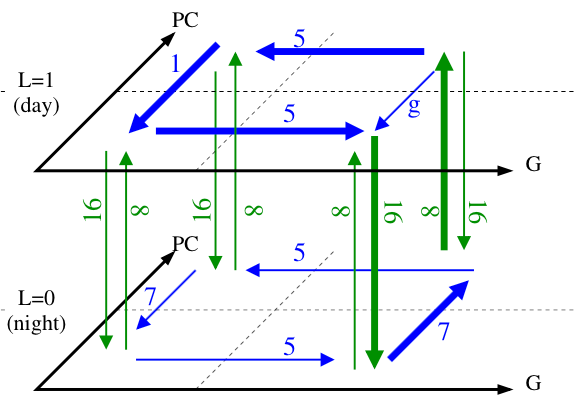
\includegraphics[width=0.4\linewidth]{images/circadianClock-summer.png}
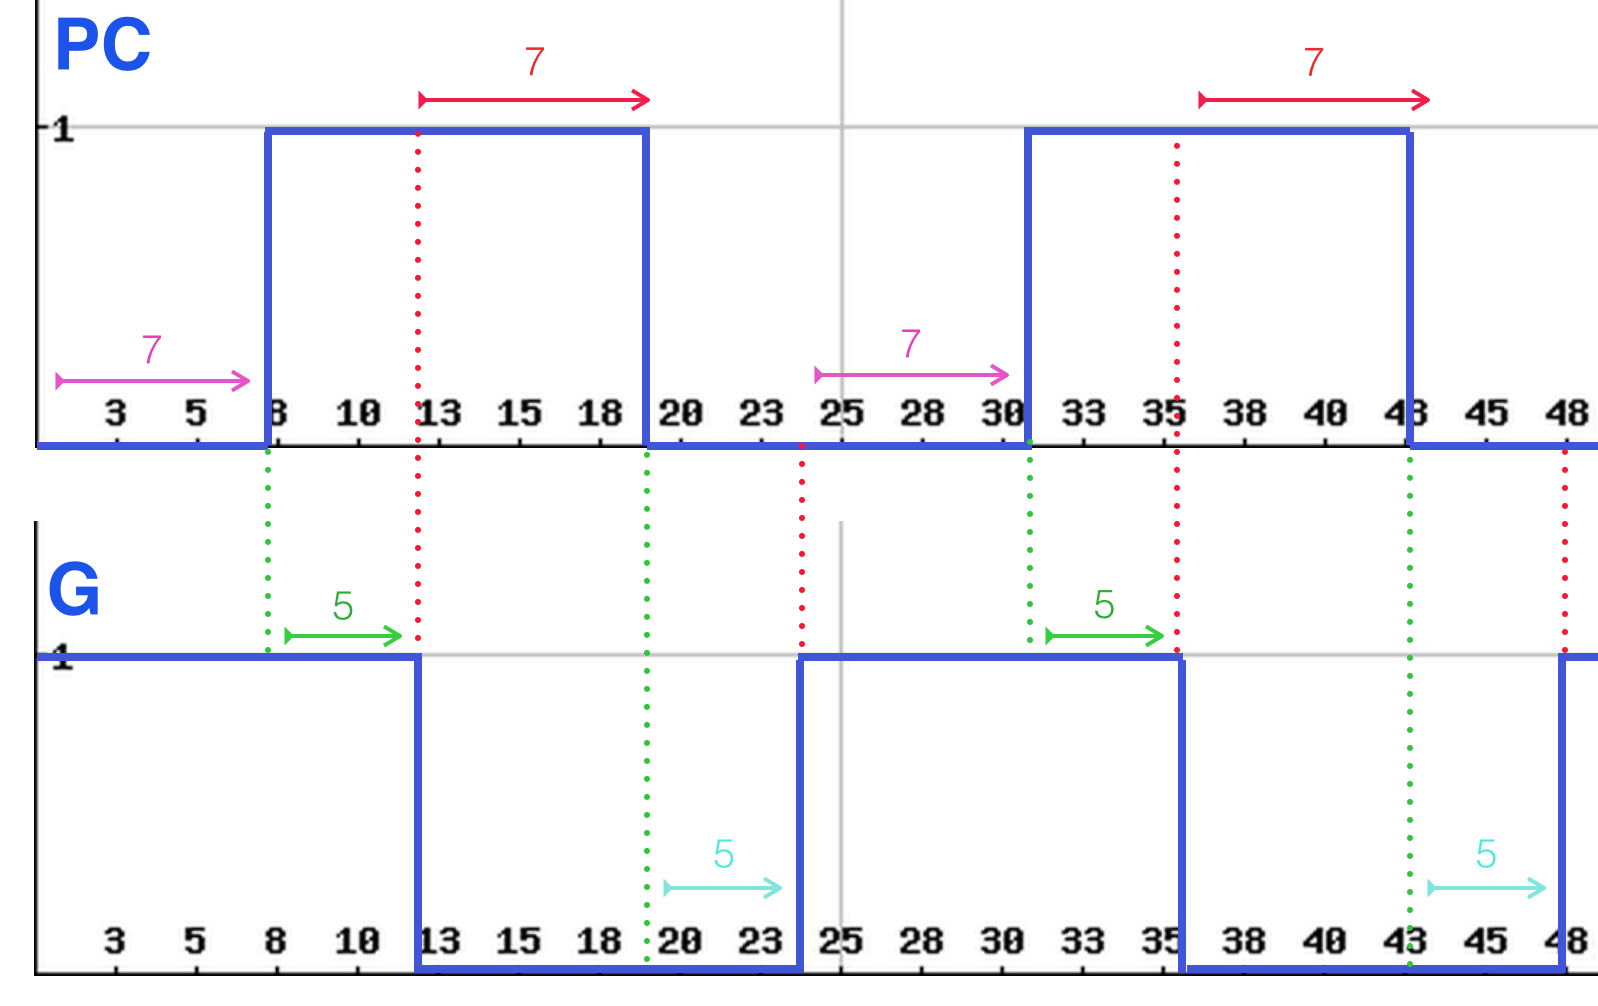
\includegraphics[width=0.4\linewidth]{images/circadianClock-Courb.png}
\end{center}
\caption{The first figure is taken from \cite{comet2010formal}, it presents the qualitative model of the mammalian circadian cycle during the summer. The second one is a chronogram corresponding to the discretization of the observed data set of a circadian clock components during the night (L=0).}
\label{fig:circadian_clock}
\end{figure}

The left part of Figure \ref{fig:PH_circadian} shows the circadian clock represented as a Process Hitting with timed plural actions.
Here, the light $L$, the gene $PC$ and $G$ are represented by sorts with two processes.
The light clock is represented by an autonomous temporized sort: there are only auto-actions.
Actions are represented by edges as follows: when a node have incoming edge its the target of an action and the hitters of this action are the nodes where those edges are coming.
Each action is labelled by its delay.
Right part of the figure shows the representation of the circadian clock with the ASP formulation we presented in section \ref{sec:ph-asp}.



\subsection{Experiments}

In this section, we evaluate our approach on learning the circadian clock actions.
All experiments are run with a ASP implementation of Algorithm \ref{alg:PHC_ap} on a processor Intel Xeon (X5650, 2.67GHz) with 12GB of RAM.

	\begin{figure}[htb!]
	\vspace{1.5cm}
	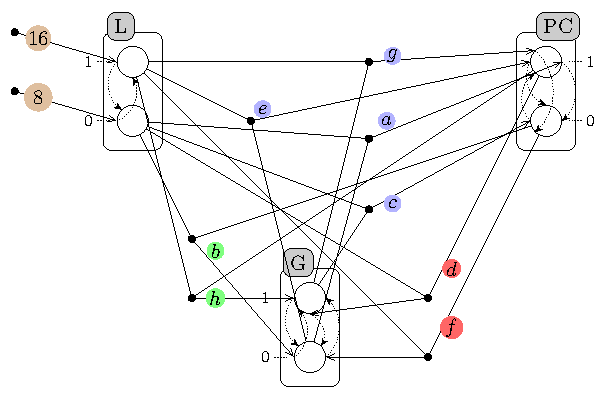
\includegraphics[width=0.6\linewidth]{images/circadianPH.pdf}
	%
	\hspace{0.1cm}
	%
	\begin{minipage}{0.32\linewidth}
	\vspace{-5cm}
		\textbf{Nodes:} \\
	\texttt{{\ssmall process("L",0..1).} }\\
	\texttt{{\ssmall process("PC",0..1).}}\\
	\texttt{{\ssmall process("G",0..1).} }\\
	\texttt{{\ssmall temporised("L").} }\\

	\textbf{Actions:} \\
	\texttt{{\ssmall action("L",0, "L",0,1,  8).}} ~\\
	\texttt{{\ssmall action("L",1, "L",1,0,  16).}} ~\\
	\texttt{{\ssmall action("L",0, "G",0, "PC",1,0,  a).}} ~\\
	\texttt{{\ssmall action("L",0, "PC",0, "G",0,1, b).}} ~\\
	\texttt{{\ssmall action("L",0, "G",1, "PC",0,1, c).}} ~\\
	\texttt{{\ssmall action("L",0, "PC",1, "G",1,0, d).}} \\
	\texttt{{\ssmall action("L",1, "G",0, "PC",1,0,  e).}} ~\\
	\texttt{{\ssmall action("L",1, "PC",0, "G",0,1, f).}} ~\\
	\texttt{{\ssmall action("L",1, "G",1, "PC",1,0, g).}} ~\\
	\texttt{{\ssmall action("L",1, "PC",1, "G",1,0, h).}} 

	\end{minipage}
	\label{fig:PH_circadian}
	\caption{Representation of circadian clock in Process Hitting (left) and the equivalent ASP representation (right). The value $"a", "b", ..., "h"$ represent the delays in actions. }
	\end{figure}
%

When the ASP representation of a chronogram like the one of Figure \ref{fig:circadian_clock} is given as input to Algorithm \ref{alg:PHC_ap} it will generate all the timed actions that can induce the observed changes.
The delay of the action is simply determined from the time delay between two changes.

\begin{figure}[htb!]
\begin{center}
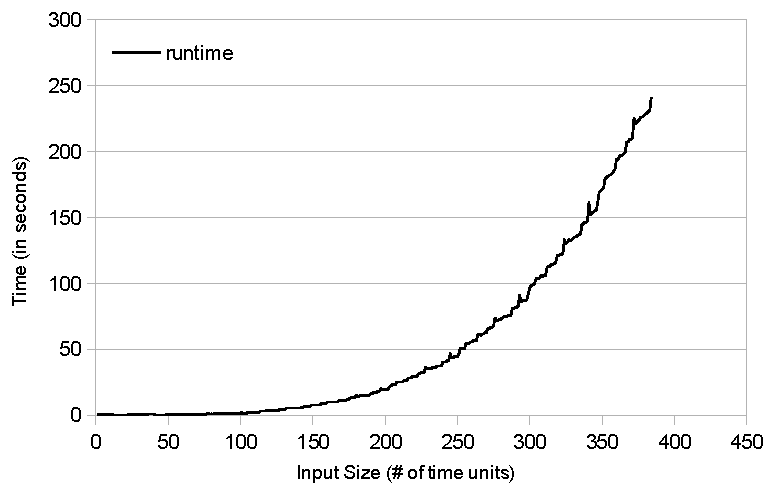
\includegraphics[width=0.5\linewidth]{images/circadian_run_time}
\end{center}
\caption{Run time of the application of Algorithm \ref{alg:PHC_ap} on circadian clock chronograms varying the number of time steps.}
\label{fig:run_time}
\end{figure}

Figure \ref{fig:run_time} shows the evolution of run time of our ASP implementation of Algorithm \ref{alg:PHC_ap} on the inference of the circadian clock actions regarding the quantity of input data.
In this experiment, we analyse the scalability of our approach by varying the the number of time units of the input, i.e. the size of the chronogram.
Here we can see that the time needed to analyse the input data grows exponentially.
The experiments stop at 384 because the memory required by the ASP solver reached the 12GB of RAM we have.
It is currently quite difficult to obtain real data from biological system with chronogram exceeding 100 points.
In work like \cite{Fippo14} the considered chronograms are only composed of about 10 points.
Regarding the circadian clock, a chronogram of 100 data points is about 4 days of data, that is not much information, especially in cases where we want to analyze the effect of perturbations (for example, understand the recoverability phase in case of jet-lag). 
% TODO Morgan: Plus de blabla
